\chapter{Diagrammes}
\label{s:Diagrammes}


\section{Diagramme des fonctionnalit�s}
\label{s:Diagramme_fonctionnalites}

\begin{figure}[htp]
   \centering
   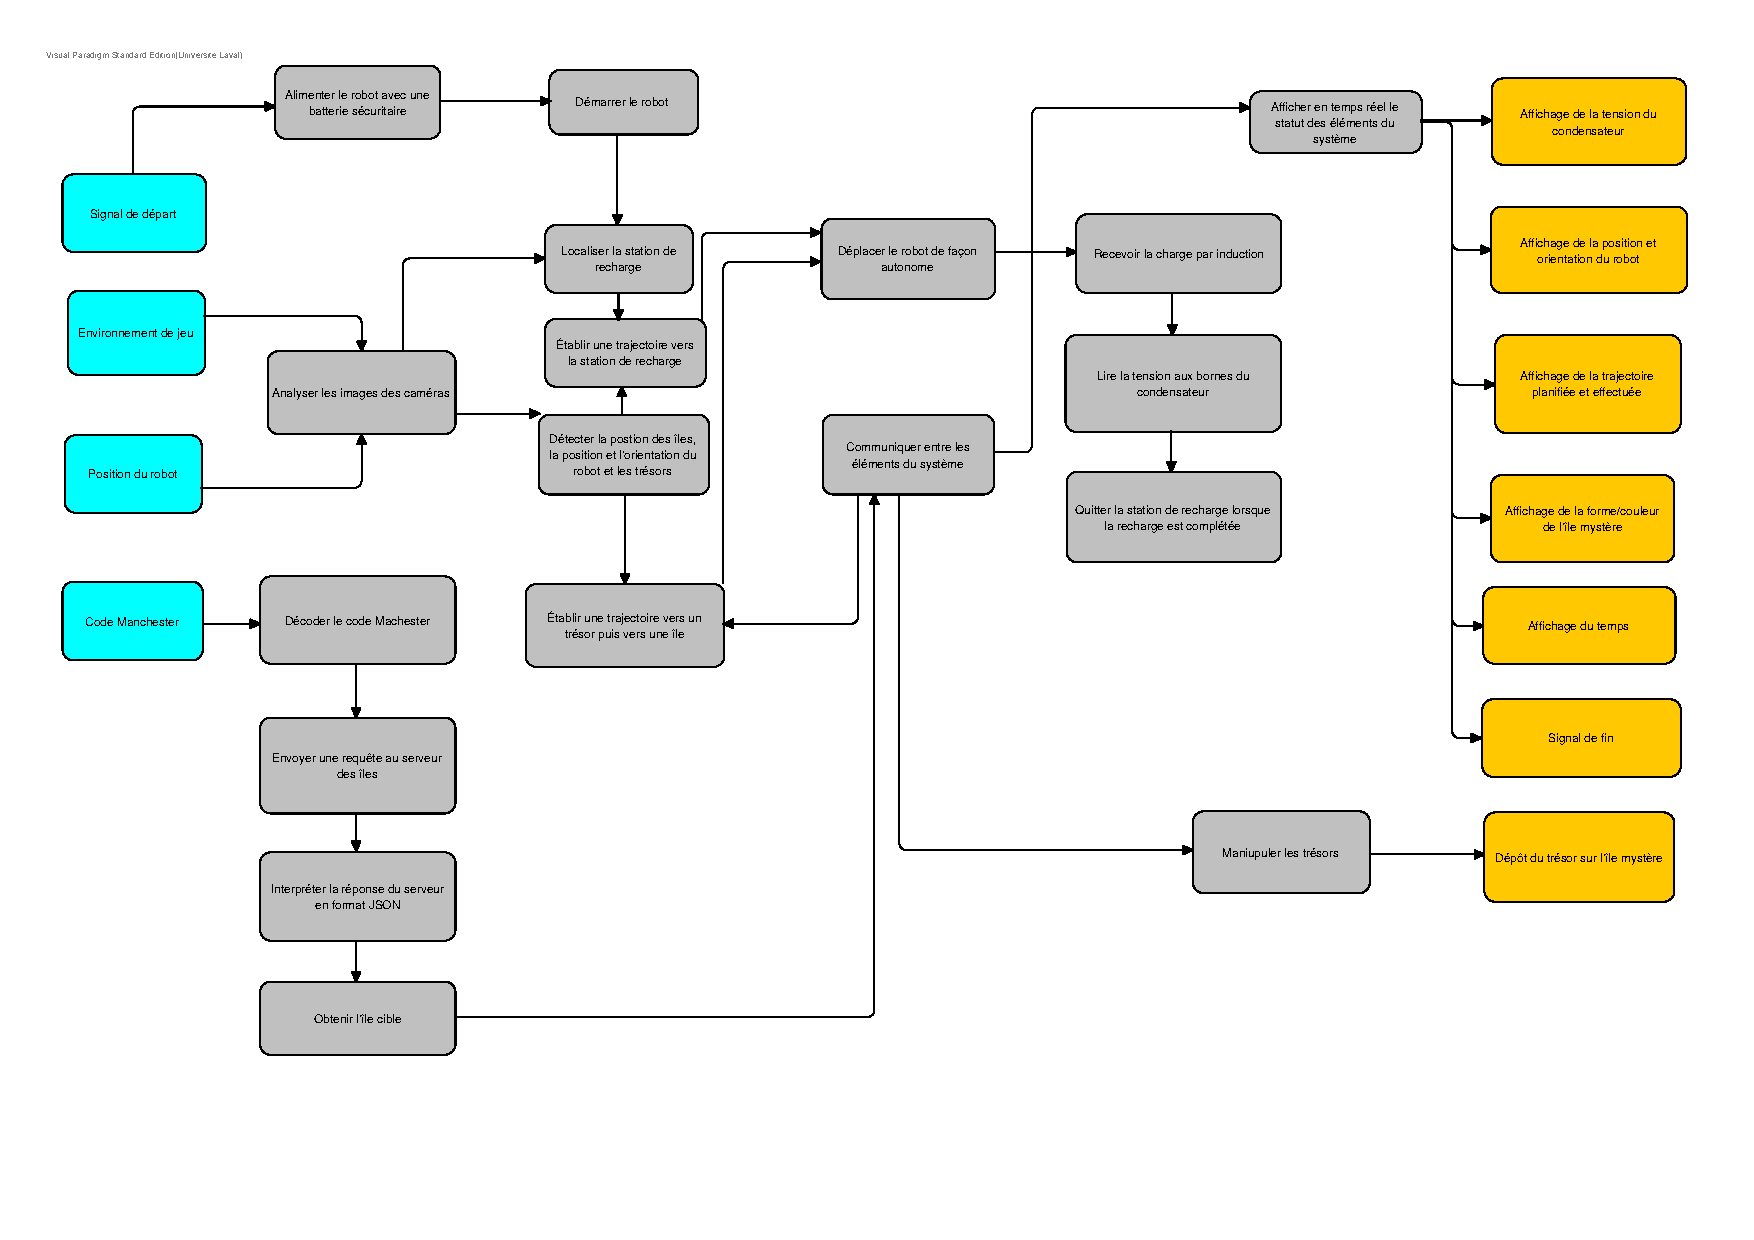
\includegraphics[width=1\textwidth]{pdf/DiagrammeFonctionnalites.pdf}
   \caption{Diagramme des fonctionnalit�s}
   \label{f:diagramme_fonctionnalites}
\end{figure}


\section{Diagramme physique}
\label{s:diagramme_physique}

\begin{figure}[htp]
   \centering
   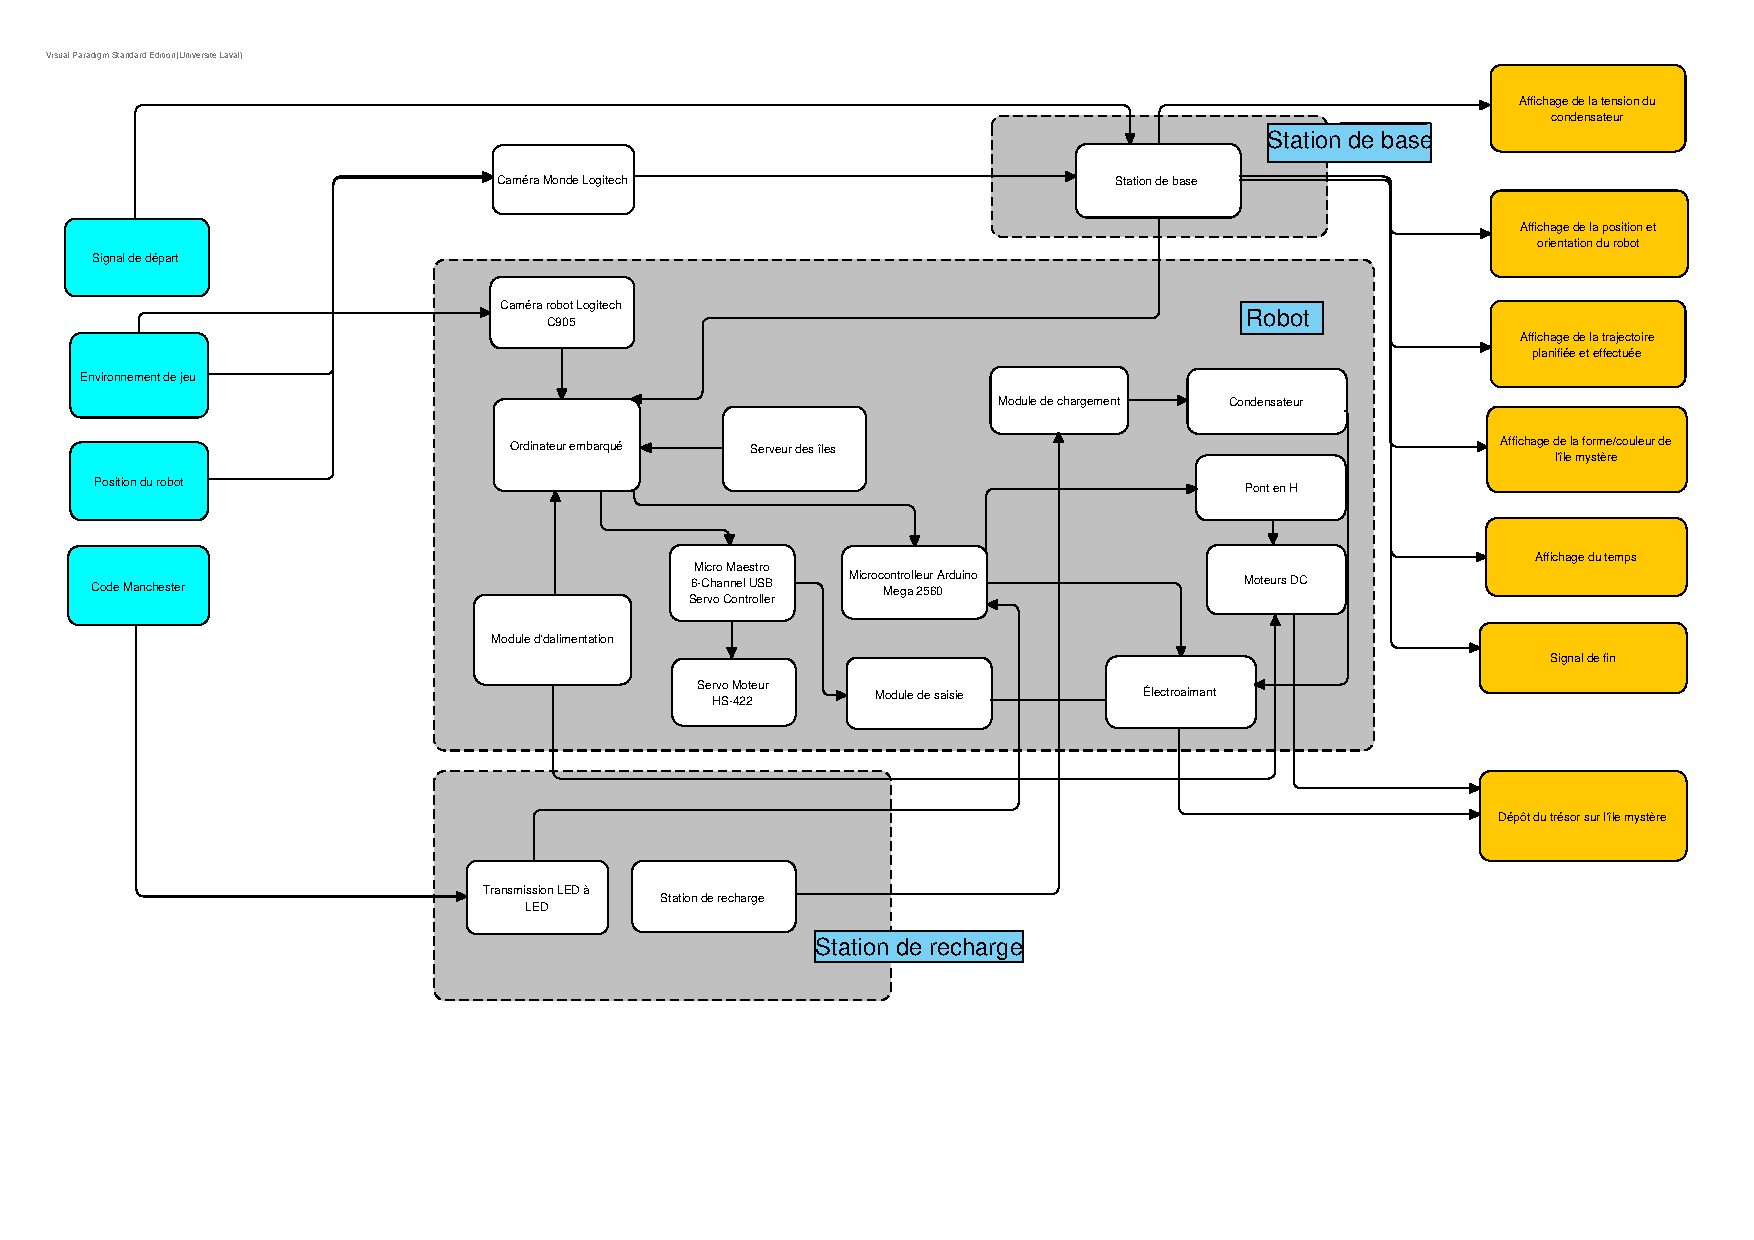
\includegraphics[width=1\textwidth]{pdf/DiagrammePhysique.pdf}
   \caption{Diagramme physique}
   \label{f:diagramme_physique}
\end{figure}


\section{Diagramme de classes}
\label{s:diagramme_classes}

%\begin{figure}[htp]
%   \centering
%   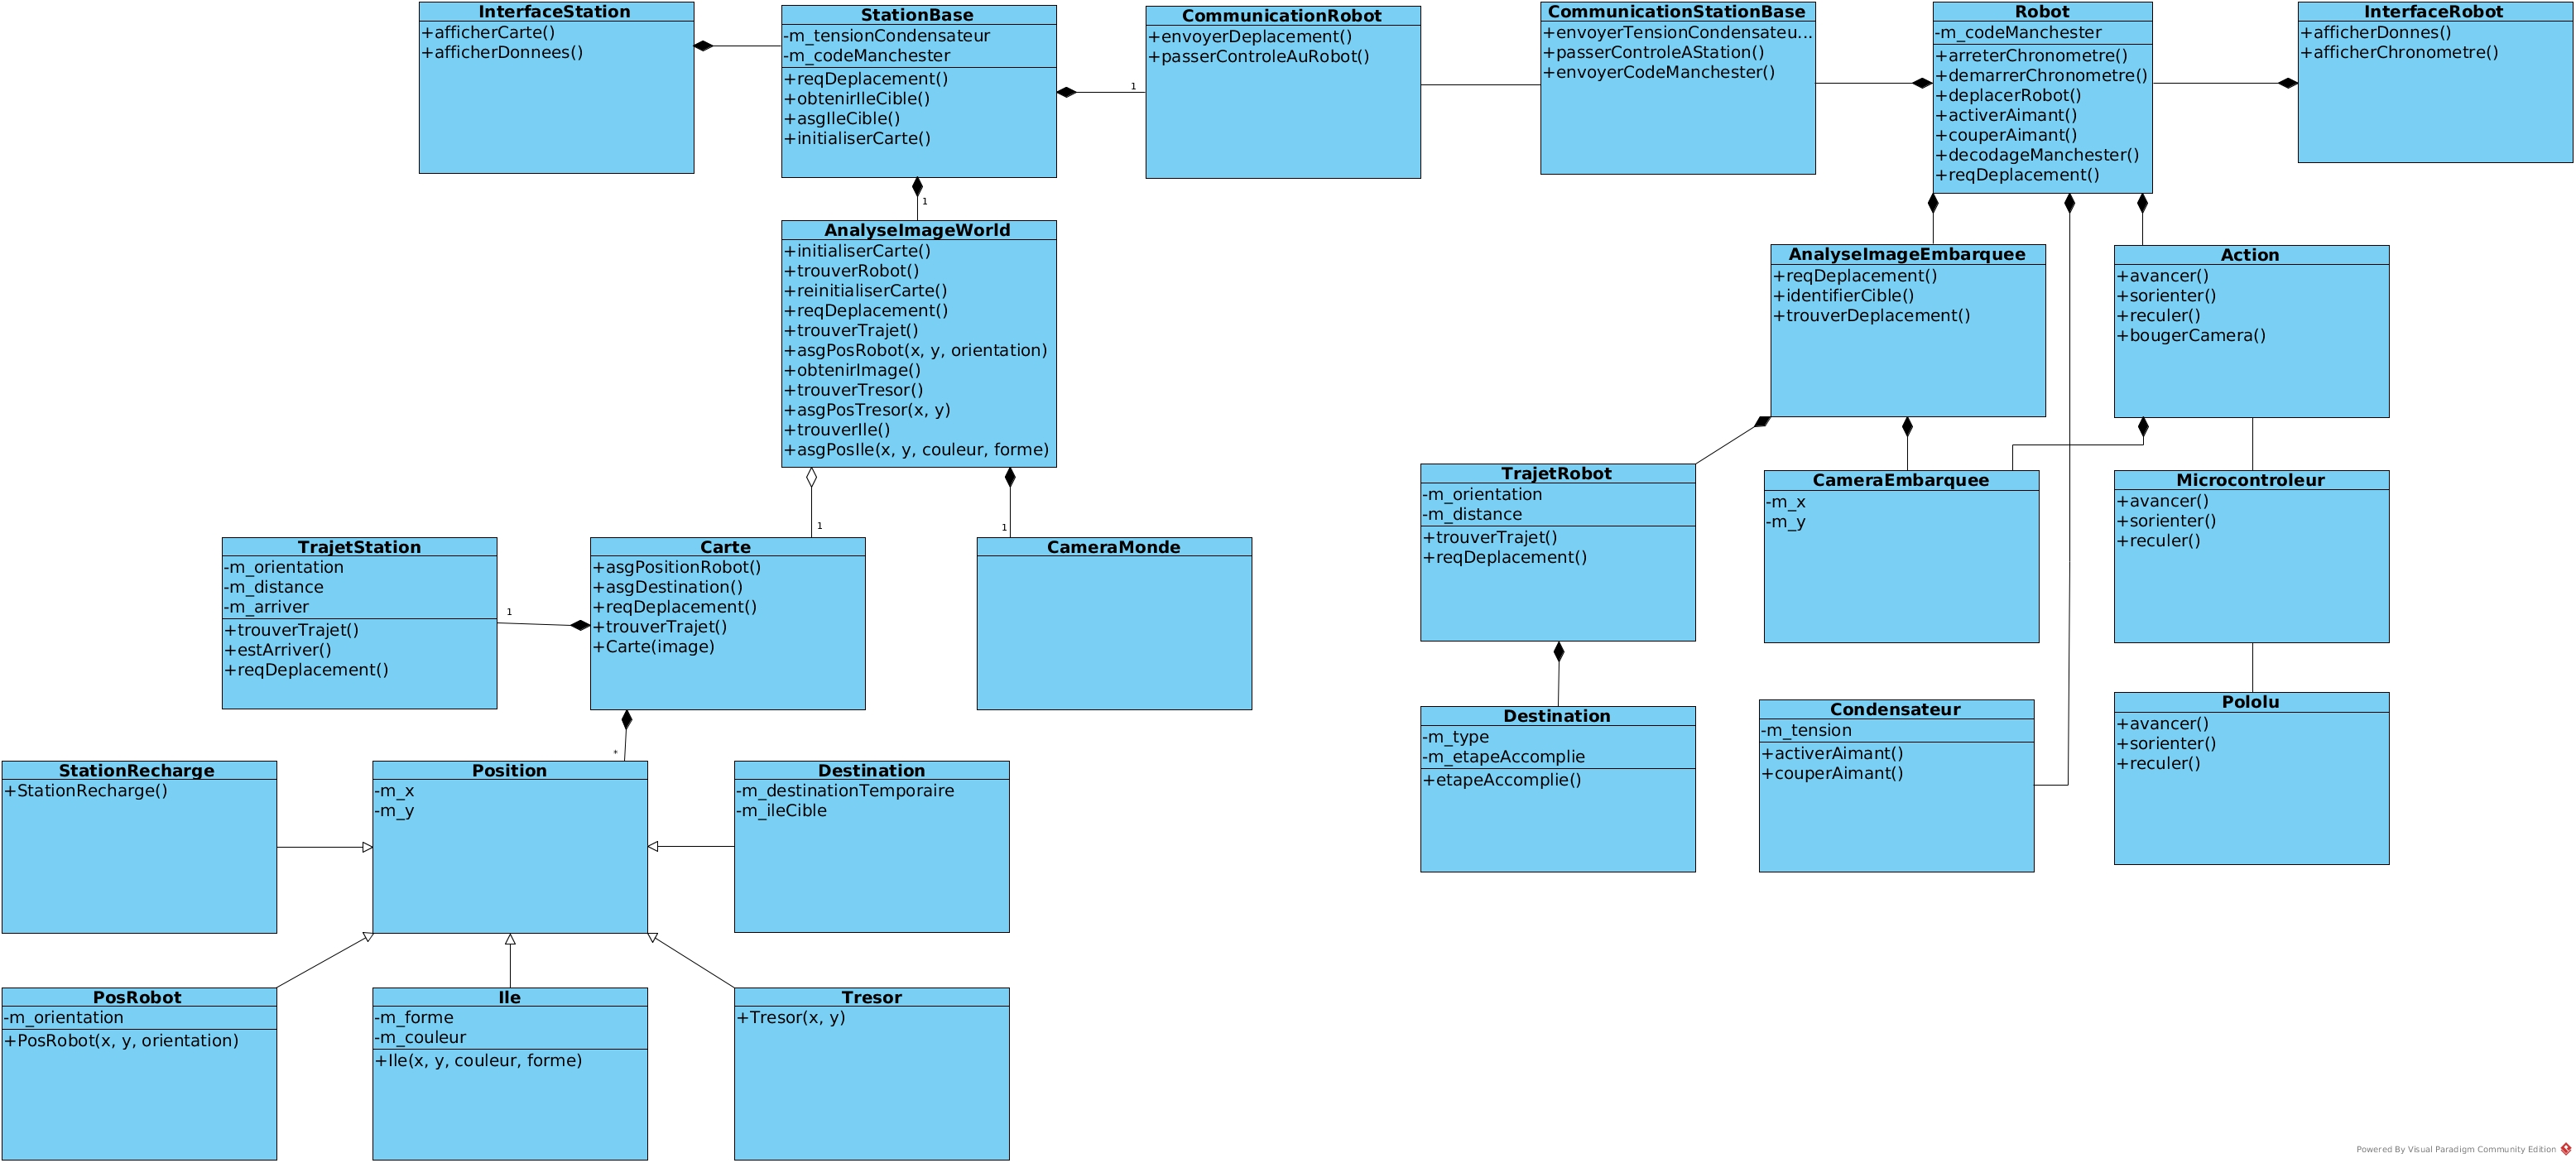
\includegraphics[width=1\textwidth]{pdf/ClassDiagram.pdf}
%   \caption{Diagramme de classes}
%   \label{f:diagramme_classes}
%\end{figure}


\section{Diagramme de s�quences}
\label{s:diagramme_sequence}

%\begin{figure}[htp]
%   \centering
%   \includegraphics[width=1\textwidth]{pdf/DiagrammeSequences.pdf}
%   \caption{Diagramme de s�quences}
%   \label{f:diagramme_sequence}
%\end{figure}
